\begin{enumerate}[label=]
    \item 
        We just have to show that the set of pull-back and terminal is the same as the set of terminal, product and equalizer.
        \begin{enumerate}[label=(\textit{\roman*})]
            \item 
                Pull-back, Terminal $\Rightarrow$ Product \newline
                If $A, B \in \mathcal C_0$ we can obtain $A \times B$ with this pull-back:
                \begin{center}
                    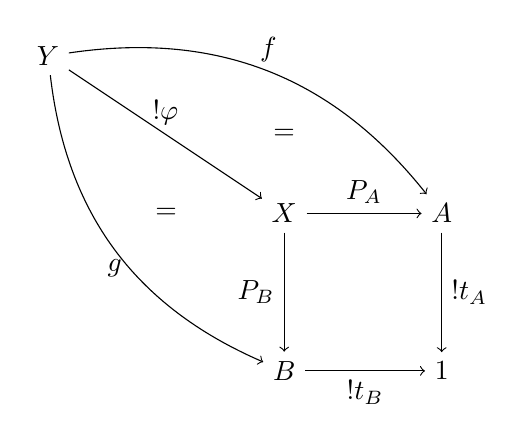
\begin{tikzpicture}
                        \node at (1, 0) (1) {$1$};
                        \node at (-1, 0)  (B) {$B$};
                        \node at (-1, 2) (X) {$X$};
                        \node at (1, 2) (A) {$A$};
                        \node at (-2.5, 2) (=) {$=$};
                        \node at (-1, 3) (=) {$=$};
                        \node at (-4, 4) (Y) {$Y$};

                        \path [->]
                            (Y) edge [above, bend left=30] node {$f$} (A)
                            (Y) edge [below, bend right] node {$g$} (B)
                            (A) edge [right] node {$!t_A$} (1)
                            (B) edge [below] node {$!t_B$} (1)
                            (Y) edge [above] node {$!\varphi$} (X)
                            (X) edge [left]  node {$P_B$} (B)
                            (X) edge [above] node {$P_A$} (A);
                    \end{tikzpicture}
                \end{center}
                Since for any $f$ and $g$ the diagram commutes since 1 is terminal object and there is only one morphism from $Y$ to 1. And since $X$ is the pull-back then there exists a unique morphism from $Y$ to $X$ such that it commutes with $f$ and $g$.
                This shows that $X$ is the product of $A$ and $B$.
            \item 
                Pull-back $\Rightarrow$ Equalizer \newline
                Consider the product $B\times B$. We want to find the equalizer of $f, g: A \to B$.
                Let $X$ be the pull-back of $\braket{f, g}$ and $\braket{id, id}$.
                \begin{center}
                    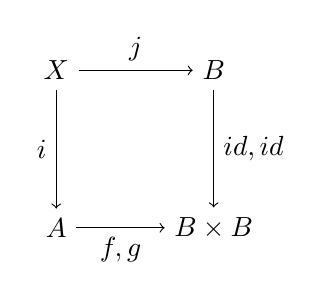
\begin{tikzpicture}
                        \node at (0, 0) (A) {$A$};
                        \node at (2, 0) (BB) {$B \times B$};
                        \node at (0, 2) (X) {$X$};
                        \node at (2, 2) (B) {$B$};

                        \path [->] 
                            (X) edge [left] node {$i$} (A)
                            (X) edge [above] node {$j$} (B)
                            (B) edge [right] node {$\braket{id, id}$} (BB)
                            (A) edge [below] node {$\braket{f, g}$} (BB);
                    \end{tikzpicture}
                \end{center}
                With $\braket{f, g}i = \braket{id, id }j$. Where $\braket{f, g}$ and $\braket{id, id}$ are defined below.
                \begin{center}
                    \begin{tikzpicture}
                        \node at (0, 0) (1) {$B$};
                        \node at (3.5, 0) (2) {$B \times B$};
                        \node at (7, 0) (3) {$B$};
                        \node at (3.5, 3) (4) {$B$};
                        \node at (8, 0) (5) {$B$};
                        \node at (11.5, 0) (6) {$B \times B$};
                        \node at (15, 0) (7) {$B$};
                        \node at (11.5, 3) (8) {$A$};
                        \node at (3.5, 6) (X1) {$X$};
                        \node at (11.5, 6) (X2) {$X$};
                        
                        \path [->] 
                            (X1) edge [left] node {$j$} (1)
                            (X1) edge [right] node {$j$} (3)
                            (X2) edge [left] node {$gi$} (5)
                            (X2) edge [right] node {$fi$} (7)
                            (X1) edge [right] node {$j$} (4)
                            (X2) edge [right] node {$i$} (8)
                            (8) edge [right] node {$\braket{f, g}$} (6)
                            (6) edge [below] node {$P_2$} (7)
                            (6) edge [below] node {$P_1$} (5)
                            (8) edge [above] node {$f$} (7)
                            (8) edge [above] node {$g$} (5)
                            (4) edge [right] node {$\braket{id, id}$} (2)
                            (2) edge [below] node {$P_2$} (3)
                            (2) edge [below] node {$P_1$} (1)
                            (4) edge [above] node {$id$} (3)
                            (4) edge [above] node {$id$} (1);
                    \end{tikzpicture}
                \end{center}
                First we show that $fi = gi$. Since both of these diagrams commute then we know that $j = P_1 \braket{id, id } j = P_2 \braket{id, id} j$. 
                Now we can replace $\braket{id, id }j$ with $\braket{f, g } i$.
                \begin{gather*}
                    P_1 \braket{f, g }i = P_2 \braket{f, g } i
                \end{gather*}
                But we know $gi = P_1 \braket{f, g } i $ and $fi = P_2 \braket{f, g }i$.
                This shows that $gi = fi$. \newline
                Now let $(Z, \varphi)$ in a way that $Z \overset{\varphi }{\to } A$ and $f\varphi = g\varphi$ where $f\varphi$ is a morphism from $Z$ to $B$. 
                we want to show that $\braket{id, id} f \varphi = \braket{f, g} \varphi$.
                since both are morphisms from $Z$ to $B \times B$ and they both commute with the diagram below, and since product is unique then they are equal.
                \begin{center}
                    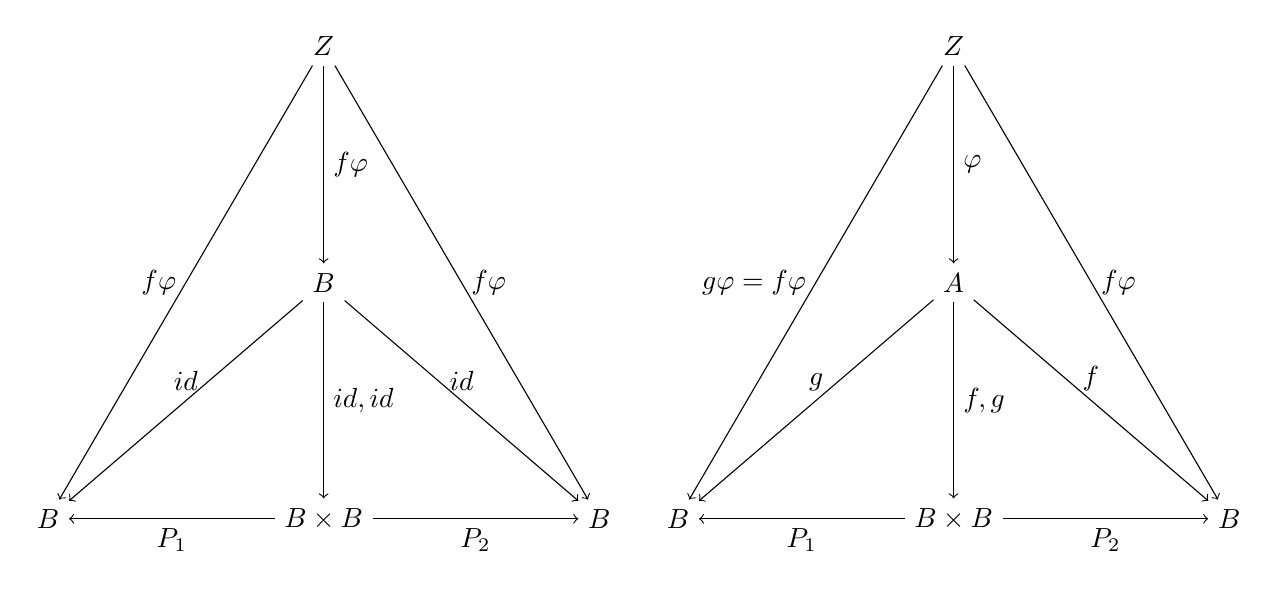
\begin{tikzpicture}
                        \node at (0, 0) (1) {$B$};
                        \node at (3.5, 0) (2) {$B \times B$};
                        \node at (7, 0) (3) {$B$};
                        \node at (3.5, 3) (4) {$B$};
                        \node at (8, 0) (5) {$B$};
                        \node at (11.5, 0) (6) {$B \times B$};
                        \node at (15, 0) (7) {$B$};
                        \node at (11.5, 3) (8) {$A$};
                        \node at (3.5, 6) (X1) {$Z$};
                        \node at (11.5, 6) (X2) {$Z$};
                        
                        \path [->] 
                            (X1) edge [left] node {$f \varphi$} (1)
                            (X1) edge [right] node {$f \varphi$} (3)
                            (X2) edge [left] node {$g \varphi = f \varphi$} (5)
                            (X2) edge [right] node {$f \varphi$} (7)
                            (X1) edge [right] node {$f \varphi$} (4)
                            (X2) edge [right] node {$\varphi$} (8)
                            (8) edge [right] node {$\braket{f, g}$} (6)
                            (6) edge [below] node {$P_2$} (7)
                            (6) edge [below] node {$P_1$} (5)
                            (8) edge [above] node {$f$} (7)
                            (8) edge [above] node {$g$} (5)
                            (4) edge [right] node {$\braket{id, id}$} (2)
                            (2) edge [below] node {$P_2$} (3)
                            (2) edge [below] node {$P_1$} (1)
                            (4) edge [above] node {$id$} (3)
                            (4) edge [above] node {$id$} (1);
                    \end{tikzpicture}
                \end{center}
                Since they are the same diagram then $\braket{id, id } f \varphi = \braket{f, g } \varphi$. then $Z$ commutes with pull-back diagram and therefore there exists a unique morphism ($\theta$) from $Z$ to $X$ in a way that $i \theta = \varphi$.
                \begin{center}
                    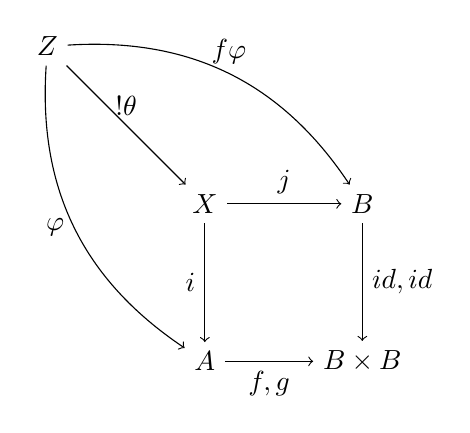
\begin{tikzpicture}
                        \node at (0, 0) (A) {$A$};
                        \node at (2, 0) (BB) {$B \times B$};
                        \node at (0, 2) (X) {$X$};
                        \node at (2, 2) (B) {$B$};
                        \node at (-2, 4) (Z) {$Z$};

                        \path [->] 
                            (Z) edge [above, bend left] node {$f \varphi$} (B)
                            (Z) edge [left, bend right] node {$ \varphi$} (A)
                            (Z) edge [above] node {$!\theta$} (X)
                            (X) edge [left] node {$i$} (A)
                            (X) edge [above] node {$j$} (B)
                            (B) edge [right] node {$\braket{id, id}$} (BB)
                            (A) edge [below] node {$\braket{f, g}$} (BB);
                    \end{tikzpicture}
                \end{center}
                this shows that $(X, i)$ is the equalizer of $f, g$.
            \item 
                Product, Equalizer $\Rightarrow$ Pull-back \newline
                This part is similar to the proof of limit, with equalizer and product.
                Suppose $f: A \to C$ and $g: B \to C$. Let $X = A \times B$. and let $(E, i)$ be the equalizer of $f P_A$ and $g P_B$.
                \begin{center}
                    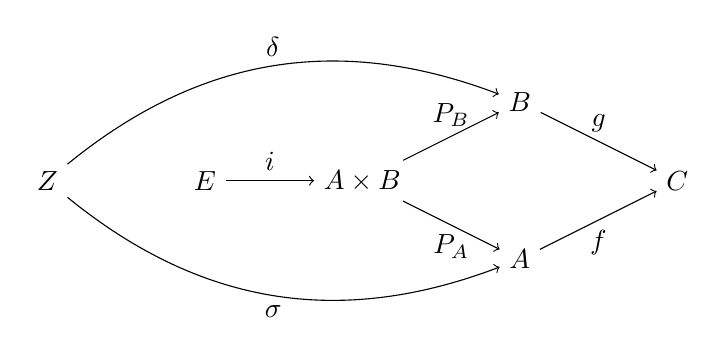
\begin{tikzpicture}
                        \node at (0, 1) (E) {$E$};
                        \node at (2, 1) (X) {$A \times B$};
                        \node at (4, 0) (A) {$A$};
                        \node at (4, 2) (B) {$B$};
                        \node at (6, 1) (C) {$C$};
                        \node at (-2, 1) (Z) {$Z$};

                        \path [->]
                            (Z) edge [above, bend left] node {$\delta$} (B)
                            (Z) edge [below, bend right] node {$\sigma$} (A)
                            (B) edge [above] node {$g$} (C)
                            (A) edge [below] node {$f$} (C)
                            (X) edge [below] node {$P_A$} (A)
                            (X) edge [above] node {$P_B$} (B)
                            (E) edge [above] node {$i$} (X);
                    \end{tikzpicture}
                \end{center}
                $E$ is the pull-back. it is easy to see that $g P_B i = f P_A i$ since $E$ is the equalizer. this shows that the diagram commutes.
                Now for any $Z$ such that commutes with this diagram, There exists a unique morphism ($\varphi$) from $Z$ to $A \times B$ such that the diagram commutes.
                \begin{gather*}
                    g \delta = f \sigma \\
                    \implies g P_B \varphi = f P_A \varphi 
                \end{gather*}
                this shows that $\varphi$ also makes $g P_B$ and $ f P_A$ equal.
                since $E$ is the equalizer then there exists a unique morphism from $Z$ to $E$ such that the diagram commutes. Therefore $E$ is the pull-back for $f$ and $g$.
        \end{enumerate}
\end{enumerate}